\documentclass[11pt,twocolumn]{article}

\usepackage[utf8]{inputenc}
\usepackage[T1]{fontenc}
\usepackage{times}
\usepackage{amsmath,amssymb,amsfonts}
\usepackage{graphicx}
\usepackage{booktabs}
\usepackage{hyperref}
\usepackage{xcolor}
\usepackage{listings}
\usepackage[margin=0.9in]{geometry}
\usepackage{enumitem}
\usepackage{tikz}
\usetikzlibrary{positioning, arrows.meta, shapes.geometric, calc, fit, backgrounds}

\setlength{\columnsep}{0.3in}
\renewcommand{\topfraction}{0.85}
\renewcommand{\textfraction}{0.15}
\hyphenpenalty=500

\hypersetup{colorlinks=true,linkcolor=blue,citecolor=blue,urlcolor=blue}
\lstset{basicstyle=\ttfamily\footnotesize,breaklines=true,frame=single,backgroundcolor=\color{gray!10}}
\setlist{nosep,leftmargin=*}

% Custom colors
\definecolor{localgreen}{RGB}{39,174,96}
\definecolor{apiblue}{RGB}{52,152,219}
\definecolor{warnred}{RGB}{231,76,60}

\title{TELOS Provider Architecture\\Technical Reference}

\author{TELOS AI Labs Inc.\\[4pt]\url{https://github.com/TELOS-Labs-AI/telos}}
\date{February 2026}

\begin{document}
\maketitle

% ============================================================================
% ABSTRACT
% ============================================================================
\begin{abstract}
This document provides a technical reference for the TELOS provider architecture, detailing the separation between local computation and external API calls. All governance mathematics---fidelity calculation, zone classification, and escalation decisions---execute locally using open-source embedding models. External APIs are used exclusively for chat completion (response generation). This architecture enables full validation of governance claims without API credentials and supports embedding provider interchangeability.
\end{abstract}

% ============================================================================
% 1. ARCHITECTURE OVERVIEW
% ============================================================================
\section{Architecture Overview}

TELOS separates \textbf{governance computation} from \textbf{response generation}:

\begin{center}
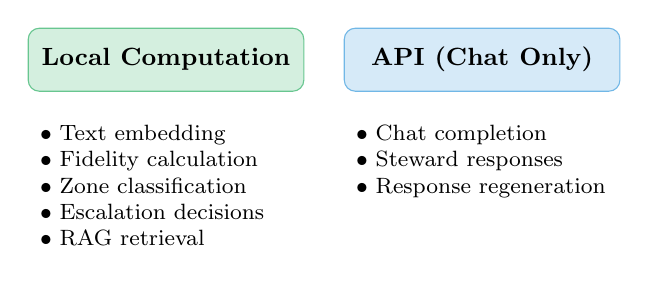
\begin{tikzpicture}[
    box/.style={rectangle, draw, rounded corners, minimum width=3.5cm, minimum height=0.8cm, align=center, font=\small},
    localbox/.style={box, fill=localgreen!20, draw=localgreen!70},
    apibox/.style={box, fill=apiblue!20, draw=apiblue!70}
]
\node[localbox] (local) {\textbf{Local Computation}};
\node[apibox, right=0.5cm of local] (api) {\textbf{API (Chat Only)}};

\node[below=0.3cm of local, font=\footnotesize, align=left, text width=3.2cm] {
    $\bullet$ Text embedding\\
    $\bullet$ Fidelity calculation\\
    $\bullet$ Zone classification\\
    $\bullet$ Escalation decisions\\
    $\bullet$ RAG retrieval
};

\node[below=0.3cm of api, font=\footnotesize, align=left, text width=3.2cm] {
    $\bullet$ Chat completion\\
    $\bullet$ Steward responses\\
    $\bullet$ Response regeneration
};
\end{tikzpicture}
\end{center}

\subsection{Design Principles}

\begin{enumerate}
    \item \textbf{Governance decisions precede API calls.} The system determines intervention level before any external request.
    \item \textbf{Embedding models are interchangeable.} The fidelity interface accepts any provider implementing \texttt{encode(text) -> ndarray}.
    \item \textbf{Validation requires no credentials.} All governance tests run with local models only.
\end{enumerate}

% ============================================================================
% 2. DATA FLOW
% ============================================================================
\section{Data Flow}

Figure~\ref{fig:provider-flow} illustrates the complete processing pipeline with local and API components marked.

\begin{figure*}[t]
\centering
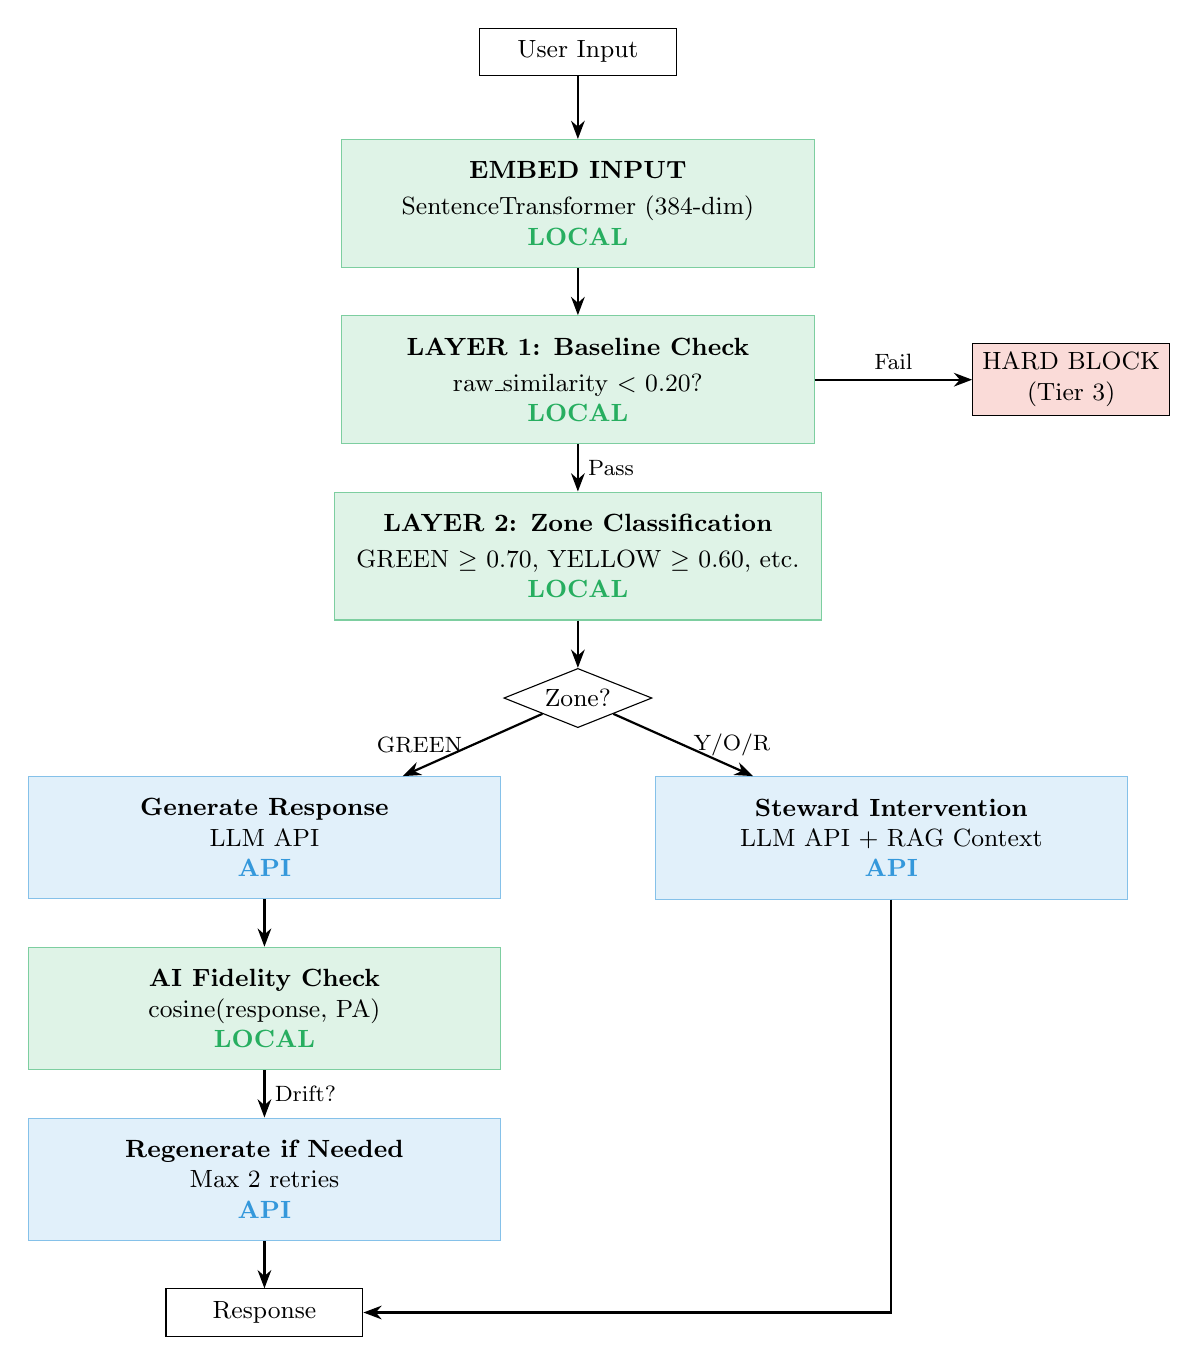
\begin{tikzpicture}[
    >=Stealth,
    node distance=0.6cm,
    box/.style={rectangle, draw, minimum width=6cm, align=center, inner sep=8pt, font=\small},
    localbox/.style={box, fill=localgreen!15, draw=localgreen!60},
    apibox/.style={box, fill=apiblue!15, draw=apiblue!60},
    decisionbox/.style={diamond, draw, aspect=2.5, inner sep=2pt, font=\small},
    smallbox/.style={rectangle, draw, minimum width=2.5cm, minimum height=0.6cm, align=center, font=\small},
    arrow/.style={->, thick}
]

% Input
\node[smallbox] (input) {User Input};

% Step 1: Embedding
\node[localbox, below=0.8cm of input] (embed) {
    \textbf{EMBED INPUT}\\[2pt]
    SentenceTransformer (384-dim)\\
    \textcolor{localgreen}{\textbf{LOCAL}}
};

% Step 2: Layer 1
\node[localbox, below=0.6cm of embed] (layer1) {
    \textbf{LAYER 1: Baseline Check}\\[2pt]
    raw\_similarity $<$ 0.20?\\
    \textcolor{localgreen}{\textbf{LOCAL}}
};

% Hard block branch
\node[smallbox, fill=warnred!20, right=2cm of layer1] (hardblock) {HARD BLOCK\\(Tier 3)};

% Step 3: Layer 2
\node[localbox, below=0.6cm of layer1] (layer2) {
    \textbf{LAYER 2: Zone Classification}\\[2pt]
    GREEN $\geq$ 0.70, YELLOW $\geq$ 0.60, etc.\\
    \textcolor{localgreen}{\textbf{LOCAL}}
};

% Decision point
\node[decisionbox, below=0.6cm of layer2] (decision) {Zone?};

% Green path
\node[apibox, below left=0.8cm and 0.5cm of decision] (native) {
    \textbf{Generate Response}\\
    LLM API\\
    \textcolor{apiblue}{\textbf{API}}
};

% Intervention path
\node[apibox, below right=0.8cm and 0.5cm of decision] (steward) {
    \textbf{Steward Intervention}\\
    LLM API + RAG Context\\
    \textcolor{apiblue}{\textbf{API}}
};

% AI Fidelity check
\node[localbox, below=0.6cm of native] (aifidelity) {
    \textbf{AI Fidelity Check}\\
    cosine(response, PA)\\
    \textcolor{localgreen}{\textbf{LOCAL}}
};

% Regeneration
\node[apibox, below=0.6cm of aifidelity] (regen) {
    \textbf{Regenerate if Needed}\\
    Max 2 retries\\
    \textcolor{apiblue}{\textbf{API}}
};

% Output
\node[smallbox, below=0.6cm of regen] (output) {Response};

% Arrows
\draw[arrow] (input) -- (embed);
\draw[arrow] (embed) -- (layer1);
\draw[arrow] (layer1) -- node[right, font=\footnotesize] {Pass} (layer2);
\draw[arrow] (layer1) -- node[above, font=\footnotesize] {Fail} (hardblock);
\draw[arrow] (layer2) -- (decision);
\draw[arrow] (decision) -- node[left, font=\footnotesize] {GREEN} (native);
\draw[arrow] (decision) -- node[right, font=\footnotesize] {Y/O/R} (steward);
\draw[arrow] (native) -- (aifidelity);
\draw[arrow] (aifidelity) -- node[right, font=\footnotesize] {Drift?} (regen);
\draw[arrow] (regen) -- (output);
\draw[arrow] (steward) |- (output);

\end{tikzpicture}
\caption{Provider data flow. Green boxes execute locally; blue boxes require LLM API. All fidelity decisions complete before any API call.}
\label{fig:provider-flow}
\end{figure*}

% ============================================================================
% 3. THREE-TIER ARCHITECTURE
% ============================================================================
\section{Three-Tier Architecture}

\subsection{Tier Summary}

\begin{table}[h]
\centering
\small
\caption{Three-Tier Components}
\begin{tabular}{@{}llll@{}}
\toprule
\textbf{Tier} & \textbf{Function} & \textbf{Computation} \\
\midrule
1 & Primacy Attractor Fidelity & LOCAL \\
2 & RAG-Enhanced Steward & LOCAL + API \\
3 & Human Expert Review & N/A (flagged) \\
\bottomrule
\end{tabular}
\end{table}

\subsection{Tier 1: Fidelity Calculation}

Embedding-based similarity measurement against the user's Primacy Attractor.

\textbf{Implementation:}
\begin{lstlisting}[language=Python]
# embedding_provider.py:131-191
class SentenceTransformerProvider:
    def __init__(self, model_name=
        "all-MiniLM-L6-v2"):
        self.model = SentenceTransformer(
            model_name)
        self.dimension = 384

    def encode(self, text) -> np.ndarray:
        return self.model.encode(text)
\end{lstlisting}

\textbf{Fidelity Formula:}
\begin{equation}
    F(q) = \cos(q, \hat{a}) = \frac{q \cdot \hat{a}}{\|q\| \cdot \|\hat{a}\|}
\end{equation}

\textbf{Normalization:} SentenceTransformer returns L2-normalized vectors by default. With unit vectors, cosine similarity reduces to dot product: $F(q) = q \cdot \hat{a}$.

\subsection{Tier 2: RAG-Enhanced Review}

For ambiguous cases (fidelity 0.50--0.70), the system retrieves relevant context from a domain-specific corpus before generating a response.

\textbf{Domain Knowledge Integration:} The RAG corpus represents authoritative knowledge for a given domain. For example, a consumer brand could load product specifications, return policies, and safety guidelines; a healthcare application might include clinical protocols and regulatory requirements; a financial services deployment could incorporate compliance documentation and risk disclosures.

\textbf{Graduated Intervention vs. Binary Escalation:} Conventional chatbot architectures typically operate in two modes: scripted responses for recognized queries, and immediate escalation to human review for everything else. This creates a gap where users receive no substantive assistance before being handed off.

TELOS fills this gap through proportional control. Before human escalation (Tier 3, representing approximately 1\% of interactions), the system applies graduated interventions calibrated to the degree of drift detected:

\begin{itemize}
    \item \textbf{GREEN zone}: Native response within purpose
    \item \textbf{YELLOW zone}: Soft guidance with context injection
    \item \textbf{ORANGE zone}: Active redirect using corpus knowledge
    \item \textbf{RED zone}: Strong intervention with RAG-enhanced response
\end{itemize}

Each intervention level draws on the preloaded domain knowledge base, providing contextually appropriate assistance proportional to the detected drift. Human escalation occurs only after these substantive interventions have been exhausted---not as a first resort when queries fall outside scripted paths.

\textbf{RAG Retrieval (LOCAL):}
\begin{lstlisting}[language=Python]
# telos_corpus_loader.py:280-368
def retrieve(self, query, top_k=3):
    query_emb = self.provider.encode(query)
    sims = np.dot(self.embeddings, query_emb)
    return self.docs[np.argsort(sims)[-k:]]
\end{lstlisting}

\textbf{Similarity Distinction:}
\begin{itemize}
    \item \textbf{RAG similarity}: Corpus-relative (finding relevant knowledge)
    \item \textbf{Fidelity similarity}: Purpose-relative (alignment to user's PA)
\end{itemize}

\textbf{Response Generation (API):}
\begin{lstlisting}[language=Python]
# beta_steward_llm.py:477-483
response = self.client.chat.complete(
    model="mistral-small-latest",
    messages=messages,
    max_tokens=8000
)
\end{lstlisting}

\subsection{Tier 3: Human Review}

Automatic escalation when:
\begin{itemize}
    \item raw\_similarity $<$ 0.20 (extreme deviation)
    \item SAAI cumulative drift $>$ 20\%
    \item Safety-critical content detected
\end{itemize}

\textbf{SAAI:} Session-Accumulated Alignment Index. Cumulative sum of per-turn fidelity deltas over a sliding window (default: 5 turns).

No AI response is generated---the session is logged for expert review.

% ============================================================================
% 4. TWO-LAYER FIDELITY PIPELINE
% ============================================================================
\section{Two-Layer Fidelity Pipeline}

\subsection{Layer 1: Baseline Pre-Filter}

Catches extreme off-topic content before full zone classification.

\begin{lstlisting}[language=Python]
# beta_response_manager.py:133
if raw_similarity < SIMILARITY_BASELINE:
    return HARD_BLOCK  # Tier 3 escalation
\end{lstlisting}

Threshold: \texttt{SIMILARITY\_BASELINE = 0.20}

\subsection{Layer 2: Zone Classification}

\begin{table}[h]
\centering
\small
\caption{Fidelity Zones}
\begin{tabular}{@{}lll@{}}
\toprule
\textbf{Zone} & \textbf{Range} & \textbf{Response} \\
\midrule
GREEN & $\geq 0.70$ & Native response \\
YELLOW & 0.60--0.69 & Soft guidance \\
ORANGE & 0.50--0.59 & Redirect \\
RED & $< 0.50$ & Strong intervention \\
\bottomrule
\end{tabular}
\end{table}

Zone determination is LOCAL. Only response generation requires API.

% ============================================================================
% 5. AI RESPONSE GOVERNANCE
% ============================================================================
\section{AI Response Governance}

TELOS governs AI outputs, not just user inputs. After the LLM generates a response, the system measures its fidelity and triggers regeneration or validates correct intervention behavior depending on the user's alignment zone.

\subsection{Dual-Attractor Fidelity Model}

AI response fidelity is measured against \textit{different} attractors depending on the user's zone:

\textbf{GREEN Zone} (user fidelity $\geq$ 0.70)---Topical Alignment:
\begin{equation}
    F_{AI}(r) = \cos(\text{embed}(r), \hat{a}_{user})
\end{equation}
\begin{itemize}
    \item Reference: User's Primacy Attractor (USER\_PA)
    \item Question: Did the AI stay on the user's topic?
    \item Action: If AI drifts ($F_{AI} < 0.70$), trigger regeneration
\end{itemize}

\textbf{INTERVENTION Zones} (user fidelity $<$ 0.70)---Behavioral Alignment:
\begin{equation}
    F_{AI}(r) = \text{behavioral\_fidelity}(r, \text{expected\_band})
\end{equation}
\begin{itemize}
    \item Reference: Steward's behavioral exemplars (AI\_PA)
    \item Question: Is the AI correctly redirecting the drifted user?
    \item Action: Validate intervention matches expected behavior for zone
\end{itemize}

This dual-attractor design ensures: when users are aligned, AI serves their purpose; when users drift, AI fulfills its stewardship role with proportional intervention.

\subsection{Proportional Control System}

Intervention strength scales with drift magnitude using error signal:

\begin{lstlisting}[language=Python]
# Proportional Controller (whitepaper Section 5.3)
K_ATTRACTOR = 1.5
error_signal = 1.0 - user_fidelity
strength = min(K_ATTRACTOR * error_signal, 1.0)
\end{lstlisting}

Intervention states based on error signal:
\begin{itemize}
    \item $e < 0.30$: MONITOR (no action)
    \item $0.30 \leq e < 0.50$: CORRECT (context injection)
    \item $0.50 \leq e < 0.67$: INTERVENE (steward redirect)
    \item $e \geq 0.67$: ESCALATE (block/human review)
\end{itemize}

Response brevity is also proportional: more drift = shorter response (RED: 300 tokens, YELLOW: 500 tokens).

\subsection{Adaptive Context Thresholds}

Fidelity thresholds adapt based on conversation phase:

\begin{itemize}
    \item \textbf{Follow-up messages:} Threshold relaxes when semantic continuity is high
    \item \textbf{Drift phase:} Threshold tightens when cumulative drift detected
    \item \textbf{Recovery phase:} Threshold returns to baseline after realignment
\end{itemize}

Governance safeguards bound adaptation: thresholds never drop below hard floor (0.20), boost capped at 0.20.

\subsection{GREEN Zone: Regeneration Loop}

When user is aligned but AI drifts:

\begin{lstlisting}[language=Python]
# beta_response_manager.py:601-692
if user_fidelity >= 0.70 and ai_fidelity < 0.70:
    # User on-topic, AI drifted -> regenerate
    while ai_fidelity < 0.70 and attempt < 2:
        response = regenerate_with_guidance(
            original, user_pa, fidelity_gap)
        ai_fidelity = compute_fidelity(response)
        attempt += 1
\end{lstlisting}

\textbf{Bounded:} Max 2 retries. \textbf{Worst case:} 3 API calls.

\subsection{INTERVENTION Zones: Behavioral Validation}

When user drifts, AI generates a steward redirect. The system then validates the AI's \textit{behavior} (not topic alignment):

\begin{lstlisting}[language=Python]
# semantic_interpreter.py - Behavioral fidelity
behavioral_fidelity = compute_behavioral_fidelity(
    ai_response=steward_response,
    user_fidelity=user_fidelity  # Determines expected band
)
\end{lstlisting}

This measures whether the AI's intervention \textit{behavior} matches the expected intervention pattern for the user's drift level---not whether the response matches the user's original topic.

\textbf{All fidelity checks:} LOCAL (embedding comparison).

% ============================================================================
% 6. SCENARIO REFERENCE
% ============================================================================
\section{Scenario Reference}

\subsection{Validation (No API Required)}

\begin{table}[!htbp]
\centering
\small
\caption{Validation Scripts}
\begin{tabular}{@{}lll@{}}
\toprule
\textbf{Script} & \textbf{Embed} & \textbf{Coverage} \\
\midrule
\texttt{run\_sb243\_validation.py} & LOCAL & 50 attacks \\
\texttt{run\_xstest\_validation.py} & LOCAL & 250 prompts \\
\texttt{pytest tests/} & LOCAL & 78 tests \\
\bottomrule
\end{tabular}
\end{table}

\subsection{Dashboard Operation}

\begin{table}[!htbp]
\centering
\small
\caption{Dashboard API Usage}
\begin{tabular}{@{}lll@{}}
\toprule
\textbf{Scenario} & \textbf{Fidelity} & \textbf{API} \\
\midrule
Aligned, no drift & $\geq 0.70$ & 1 \\
Aligned, AI drifts & $\geq 0.70$ & 1--3 \\
Intervention zones & $< 0.70$ & 1 \\
Hard block & raw $< 0.20$ & 0 \\
\bottomrule
\end{tabular}
\end{table}

% ============================================================================
% 7. PROVIDER INTERFACE
% ============================================================================
\section{Provider Interface}

\subsection{Embedding Provider Contract}

Any embedding provider must implement:

\begin{lstlisting}[language=Python]
class EmbeddingProvider:
    dimension: int  # Vector dimensionality

    def encode(self, text: str) -> np.ndarray:
        """Return embedding vector."""
        ...
\end{lstlisting}

\subsection{Implemented Providers}

\vspace{0.5em}
\noindent
\begin{tabular}{@{}lll@{}}
\toprule
\textbf{Provider} & \textbf{Dim} & \textbf{Type} \\
\midrule
all-MiniLM-L6-v2 & 384 & LOCAL \\
all-mpnet-base-v2 & 768 & LOCAL \\
mistral-embed & 1024 & API \\
\bottomrule
\end{tabular}
\vspace{0.5em}

\subsection{Adding Providers}

New providers require:
\begin{enumerate}
    \item Implementation of the \texttt{encode()} interface
    \item Threshold calibration for zone boundaries
    \item Validation parity testing
\end{enumerate}

% ============================================================================
% 8. FILE REFERENCE
% ============================================================================
\section{File Reference}

\vspace{0.5em}
\noindent
\begin{tabular}{@{}lp{3.5cm}@{}}
\toprule
\textbf{Component} & \textbf{Location} \\
\midrule
Embedding providers & \texttt{embedding\_provider.py} \\
Constants & \texttt{constants.py} \\
Fidelity pipeline & \texttt{beta\_response\_manager.py} \\
RAG corpus & \texttt{telos\_corpus\_loader.py} \\
Steward LLM & \texttt{beta\_steward\_llm.py} \\
\bottomrule
\end{tabular}
\vspace{0.5em}

\noindent\textit{All files in \texttt{telos\_observatory\_v3/} directory.}

% ============================================================================
% 9. SUMMARY
% ============================================================================
\section{Summary}

\begin{itemize}
    \item All governance computation (embedding, fidelity, zone classification, escalation) executes locally.
    \item External APIs are used exclusively for chat completion.
    \item Validation scripts require no API credentials.
    \item The embedding provider interface supports model interchangeability.
    \item AI responses are governed with bounded regeneration (max 2 retries).
\end{itemize}

\vspace{1em}
\hrule
\vspace{0.5em}
\textbf{Repository:} \url{https://github.com/TELOS-Labs-AI/telos}\\
\textbf{License:} Apache 2.0

\end{document}
